\chapter*{Jak Fedoru přizpůsobit?}

\section*{Rozšíření pro GNOME Shell}
GNOME Shell disponuje rozšířeními, jež jsou mocnou zbraní co do přizpůsobení systému jednotlivému uživateli. Instalují se přímo v~prostředí webového prohlížeče z~webu \url{extensions.gnome.org}. Jedná se o~stovky rozšíření, které doplňují nebo mění jednotlivé prvky uživatelského prostředí. Změny menu, ikon, panelů, indikace, zobrazení, přepínání oken a nesčetné množství dalších.

\section*{Vylaďovací nástroj GNOME}
Aneb \emph{GNOME Tweak Tool}. Nástroj zahrnutý ve Fedoře, pomocí něhož lze podrobně, až do nejmenších detailů, nastavit jemnosti, které výchozí konfigurační nástroj neobsahuje. Můžeme zde namátkou měnit znělku prostředí, přesné chování virtuálních ploch, chování při napájení, písma aplikací, klávesové zkratky a opět desítky dalších věcí. Ostatně, můžeme zde spravovat i výše zmíněná rozšíření.

\begin{figure}[t]
\begin{center}
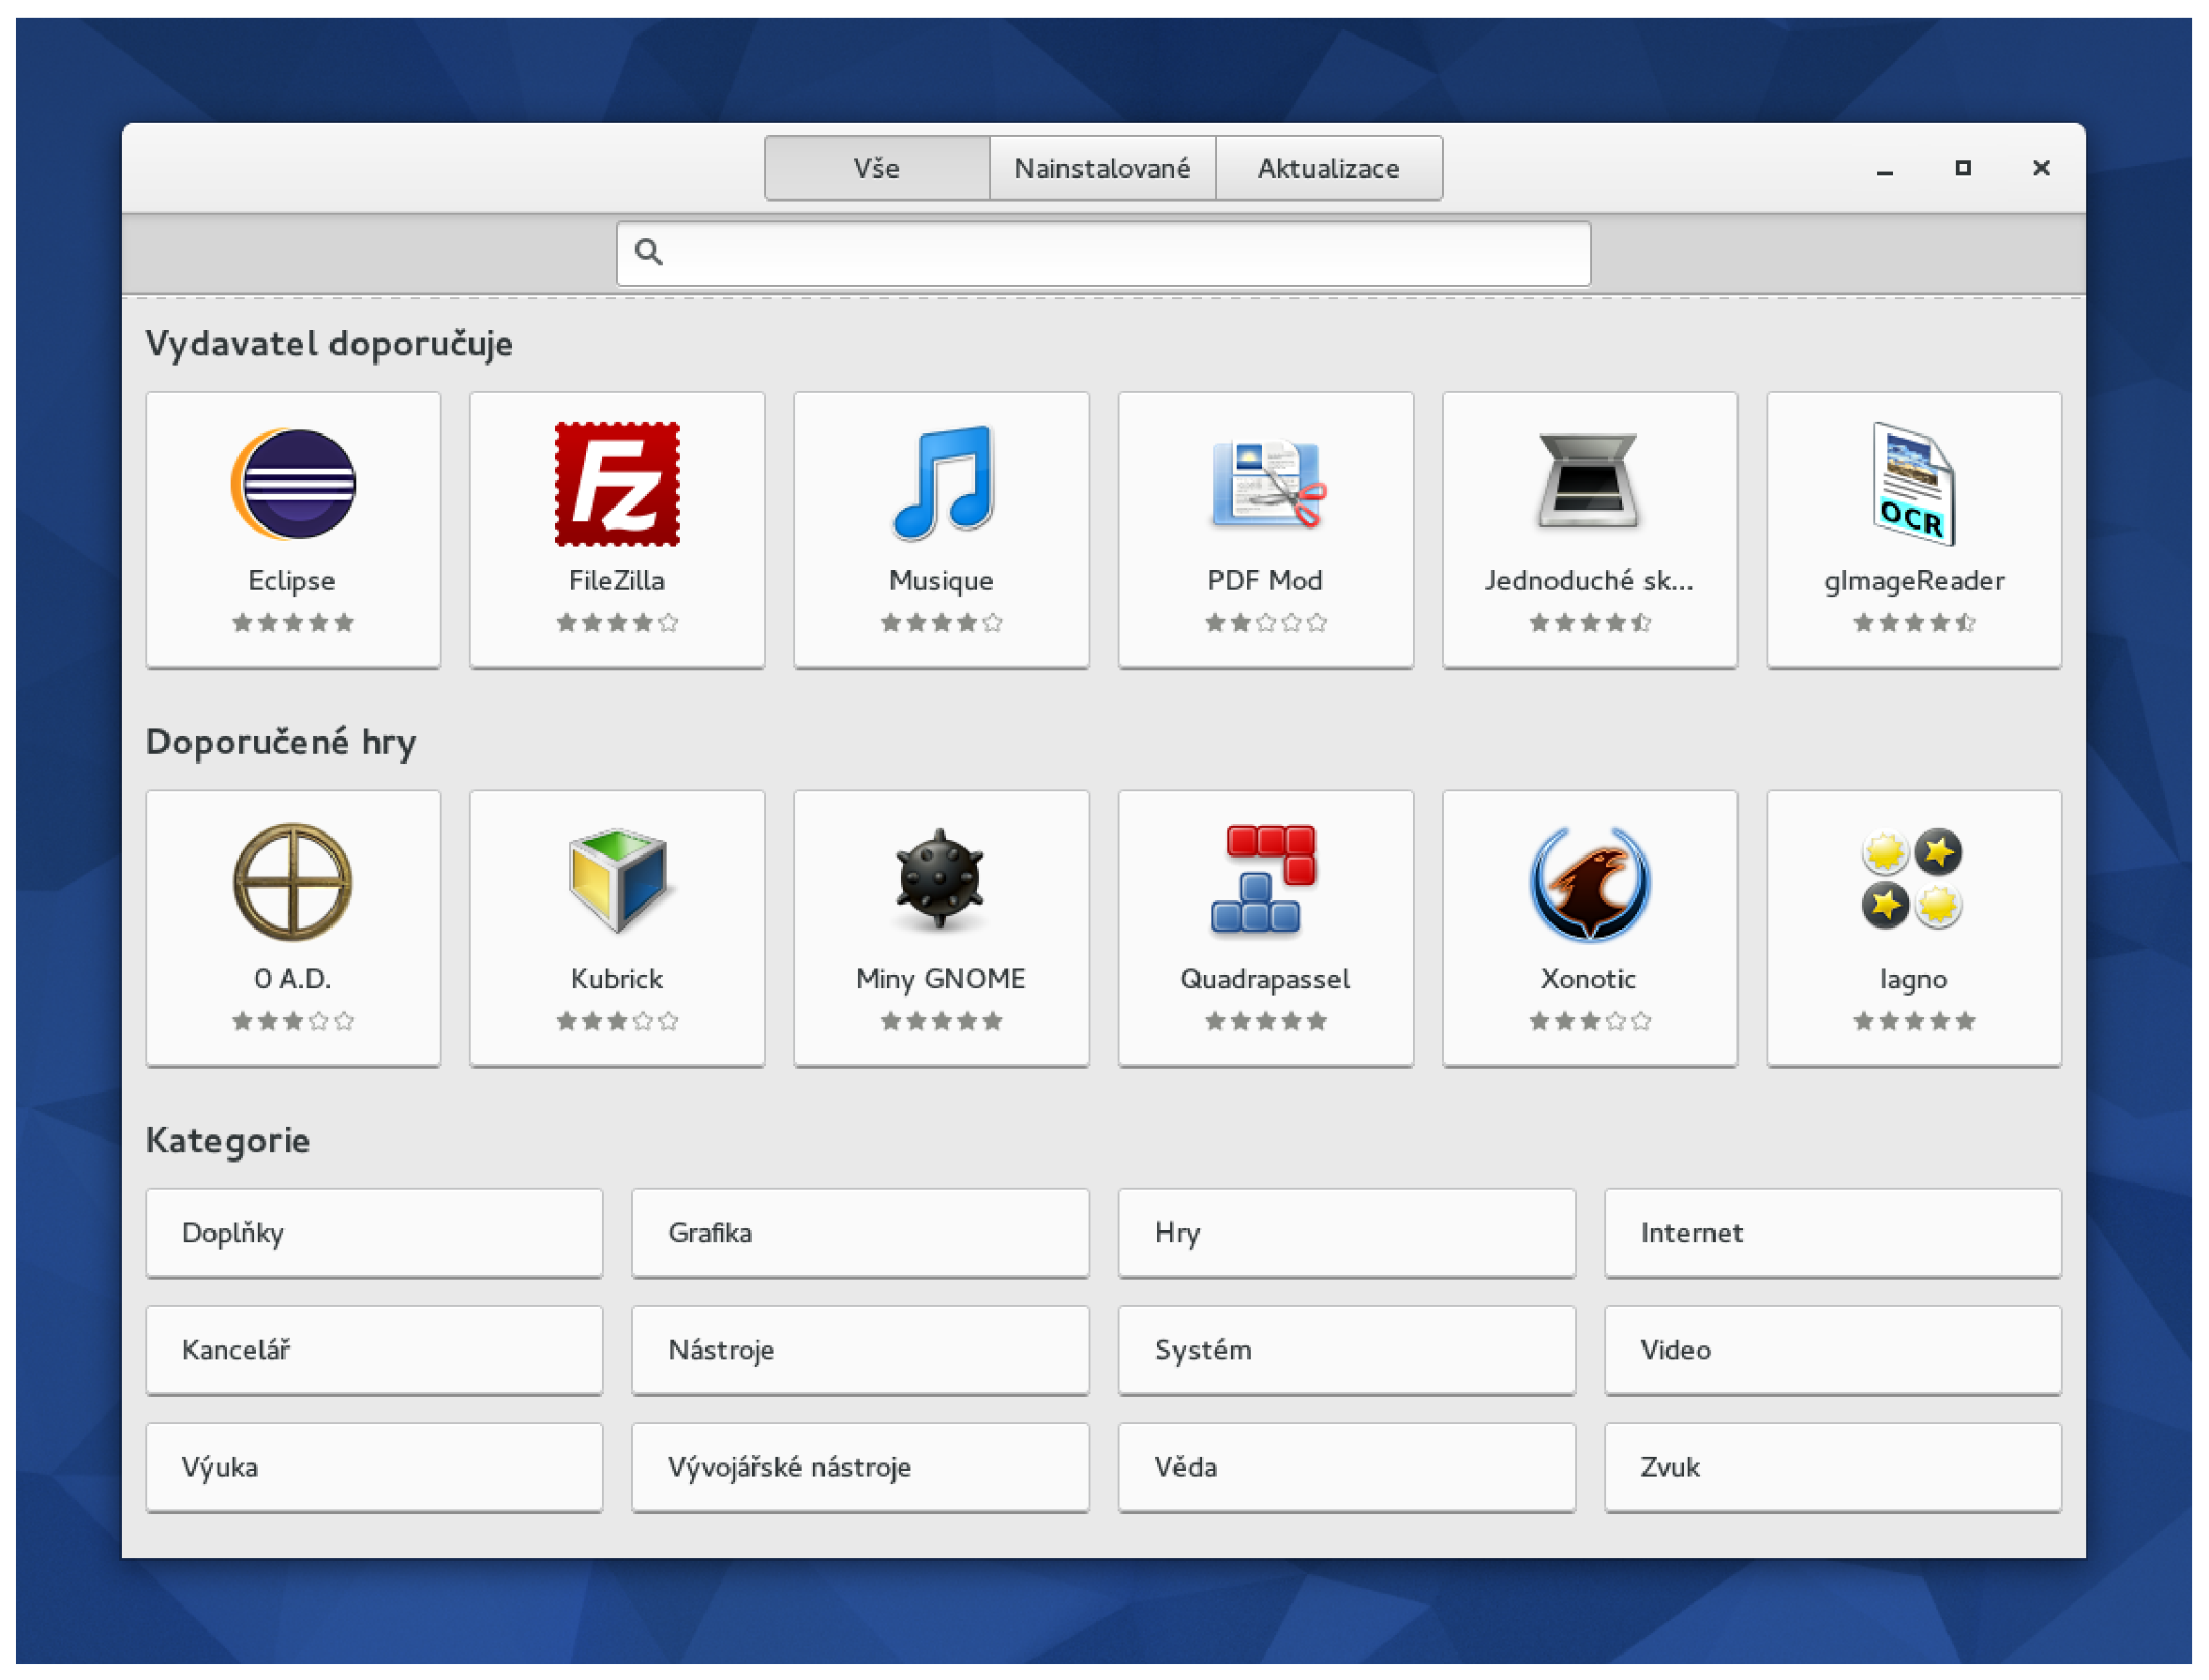
\includegraphics[width=\textwidth]{img/software}
\captionbelow{GNOME Tweak Tool} \label{fig:software}
\end{center}
\end{figure}
